\section{Scene}
In a rendering engine, the need of some kind of Scene/Scene-Graph management is unavoidable. To address this need,
\textit{SceneNodes} were created. Each node has a set of properties that define its appearance and/or behavior.
Such properties are:

\begin{itemize}
\item Key strings, used to reference assets in their respective stores (model keys, material keys).
\item A unique id to identify the node.
\item The node's category (normal node or light node).
\item The current transformation matrix of the node.
\item Node's AABBs.
\item A pointer to the parent node and a list with pointers to its child nodes.
\item Whether the node is culled or not.
\end{itemize}

\subsection{Scene Management}
Of course, having a number of SceneNodes scattered around without any management would not do any good. For that
reason, a management system is implemented. This management system shall be referred from now on as \textit{Scene}.
Scene is responsible for creating, deleting and managing the Nodes. For instance, when a node is deleted, Scene
controls what happens to its child nodes; the user may choose to delete them simultaneously with the parent node or
keep them. Identically, when a node is moved the child nodes might or might not follow it.

Another responsibility of Scene is to track any Updates and provide an interface to retrieve them. An update bundle
is created and updated every time a new node is created or an old one is deleted. The user may pull those updates
whenever required. That particular feature is utilized by the Renderer.

\subsection{Scene and Renderer}
A Renderer needs a Scene to Render. However, there is no need for the Renderer to have knowledge or even access to
details like Material Keys or Parent-Child relations. On the contrary, the ideal Scene for the Renderer is one
containing only descriptors for the GPU Resources; in OpenGL's case, integer IDs for the uploaded to GPU Resources. 

For that purpose, an Intermediate Form was created and will be referenced as \textit{IntForm} hereafter. It contains
all IDs needed by the Renderer. Those IDs are:

\begin{itemize}
\item Texture IDs for Diffuse, Normal and Specular Maps.
\item IDs for Skybox and its radiance/irradiance maps.
\item IDs of \textit{Vertex Array Objects} for each mesh. 
\item IDs of \textit{Element Buffer Objects} for each mesh.
\end{itemize}

\subsubsection{Material Sorted Scene}
It should be noted that IntForm has a container with all the Materials and their properties, ignoring each Mesh's
position and family tree in Scene Graph. All Meshes will be Rendered eventually but the order slightly varies than
the expected one.

Someone would expect that a Model will be Rendered all at once. The problem with that approach is that many materials
with their respective textures will be uploaded more than once. Peculiar as that may look, it is indeed a problem,
because that task needs to be repeated in every single frame. To eliminate that bottleneck, IntForm contains all
Meshes but when it is time for Render the order in which a Mesh will be drawn depends on its Material.

\subsection{Scenefile}
Understanding how \textit{Scene Graph} works requires knowledge on the properties file, which is referred to as
\textit{scenefile}. SceneFile helps defining material and model properties and putting them all together in a scene.
The pipeline of the whole property module is summed up in the following figure.

\begin{figure}[h]
    \centering
    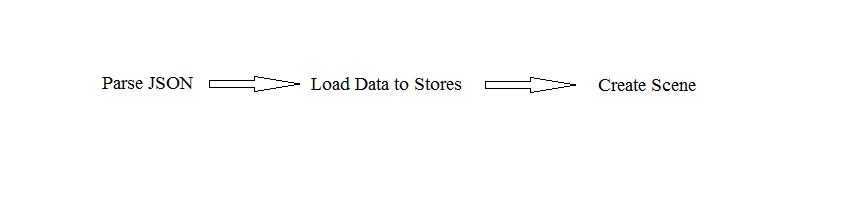
\includegraphics[scale=0.5, clip=true, trim=0 80 0 20]{./image/scene_pipeline.png}
    \caption{Scene Generation Pipeline}
\end{figure}

At its core, it is nothing more than a JSON file with various properties, inspired from three.js\cite{scene:ref1}.
It contains properties about textures, geometries, materials, models, model position in scene and whether a model
should be considered a light or not.

% Textures/Geometries
Textures and Geometries are respectivly image and model files in various formats. At the moment, the supported Image
formats are png, tga, jpg, jpeg; as for models, everything supported by Assimp library\cite{scene:ref2}.

% Models/Materials
Two other elements of the scenefile are the models and the materials. Models are nothing more than geometries with a
unique string to reference them. Materials, on the other hand, have many special properties that are used later by
our shaders. Such properties are the reflectivity, roughness, metallicity, color, normal/specular/diffuse texture
maps, etc.. It is important to note that every value is optional and have a default value in case it is ommited.

% Scenegraph
Last, but not least, there is the actual scene graph properties. An object array inside the JSON where we define
\textit{elements} we want to show in our scene. Each element gets a geometry and an array of materials. Elements of
that material array are mapped to the chosen model's meshes respectively. Additionally, a set of transformations
(scale, rotation, position) can be appended to each element, to control where it will be displayed. Every element
can have its own children and thus, the relationship tree between the nodes is formed.

\subsubsection{JSON Parsing}
All the properties are in a JSON file parsed with rapidjson\cite{scene:ref3}. The file is first loaded in memory and
then parsed all at once. When parsing comes to an end, all data are into their containers and ready to continue to
the next section of the pipeline.

\subsubsection{Loading Data}
Having everything loaded from JSON, the only task that needs to be done before composing the scene, is to load the
data to stores. Textures, Models and Materials will be loaded to thei respective stores and will be ready for future
use. When store loading is done, the scene is composed.
